\documentclass[11pt, a4paper]{article}

\usepackage[utf8]{inputenc}
\usepackage[T1]{fontenc}
\usepackage[frenchb]{babel}

\usepackage{array}
\usepackage{fancybox}
\usepackage{textcomp}
\usepackage{sectionbox}

\usepackage{fancyhdr}
\usepackage{fancyvrb}
\usepackage{titletoc}
\usepackage[hyperref,html,x11names]{xcolor}
\usepackage[colorlinks=true,pdftex=true,linkcolor=SteelBlue4]{hyperref}
\usepackage{graphicx}

%% --- Maths
\usepackage{latexsym}
\usepackage{amsfonts}
\usepackage{amssymb}

%% --- Page geometry
\textwidth 16cm
\textheight 23.5cm
\headsep 1cm
\topmargin -1.5cm
\oddsidemargin 0cm
\setlength{\unitlength}{1cm}

%% --- C#
\newcommand{\csharp}{\textsc{C\#}}

%% --- FancyHDR
\pagestyle{fancy}
\lhead{
  {\textbf{\csharp}}\\
  {\textsc{tp}} 6 -- Janvier 2014}
\rhead{
  {\small Info-Sup}\\
  {\textsc{Epita}}}
%% *** Logo
\rfoot{
\includegraphics[width=3.5cm]{../res/logo.pdf}}

%% -- Code environment (no syntax highlighting).
\newenvironment{code}%
{
\definecolor{sectboxfillcol}{rgb}{1,1,1}
\VerbatimEnvironment
\begin{center}
\framesectionbox
\small
\begin{sectionbox}[\textwidth]{}
\vspace{1mm}
\begin{Verbatim}
}%
{
\end{Verbatim}
\end{sectionbox}
\end{center}
}

%% -- XColor configuration
\hypersetup{urlcolor=cyan}

%% -- Pandoc syntax highlighting

\DefineShortVerb[commandchars=\\\{\}]{\|}
\DefineVerbatimEnvironment{Highlighting}{Verbatim}{commandchars=\\\{\}, frame=single, label=Code source, fontsize=\small}
\newenvironment{Shaded}{}{}
\newcommand{\KeywordTok}[1]{\textcolor[rgb]{0.00,0.44,0.13}{\textbf{{#1}}}}
\newcommand{\DataTypeTok}[1]{\textcolor[rgb]{0.56,0.13,0.00}{{#1}}}
\newcommand{\DecValTok}[1]{\textcolor[rgb]{0.25,0.63,0.44}{{#1}}}
\newcommand{\BaseNTok}[1]{\textcolor[rgb]{0.25,0.63,0.44}{{#1}}}
\newcommand{\FloatTok}[1]{\textcolor[rgb]{0.25,0.63,0.44}{{#1}}}
\newcommand{\CharTok}[1]{\textcolor[rgb]{0.25,0.44,0.63}{{#1}}}
\newcommand{\StringTok}[1]{\textcolor[rgb]{0.25,0.44,0.63}{{#1}}}
\newcommand{\CommentTok}[1]{\textcolor[rgb]{0.38,0.63,0.69}{\textit{{#1}}}}
\newcommand{\OtherTok}[1]{\textcolor[rgb]{0.00,0.44,0.13}{{#1}}}
\newcommand{\AlertTok}[1]{\textcolor[rgb]{1.00,0.00,0.00}{\textbf{{#1}}}}
\newcommand{\FunctionTok}[1]{\textcolor[rgb]{0.02,0.16,0.49}{{#1}}}
\newcommand{\RegionMarkerTok}[1]{{#1}}
\newcommand{\ErrorTok}[1]{\textcolor[rgb]{1.00,0.00,0.00}{\textbf{{#1}}}}
\newcommand{\NormalTok}[1]{{#1}}

\begin{document}

\begin{center}
  {\Large {\textbf{Fichiers \& Bits}}}
\end{center}

\section{Rendu}\label{rendu}

Le TP devra être rendu en réalisant une archive \texttt{zip}. Tout autre
format de fichier sera systématiquement refusé.

\subsection{Fichier \texttt{AUTHORS}}\label{fichier-authors}

Ce fichier contient votre \emph{login}, sous la forme suivante : une
étoile \texttt{*}, un espace, votre \emph{login} (\texttt{login\_x}) et
\textbf{un} retour à la ligne -- représenté par le caractère \texttt{\$}
dans l'exemple ci-dessous.

\begin{verbatim}
    * login_x$
\end{verbatim}

\subsection{Arborescence de l'archive
\texttt{zip}}\label{arborescence-de-larchive-zip}

L'archive \texttt{zip} pour ce tp se nommera
\texttt{rendu-tpcs6-login\_x.zip} et disposera de l'arborescence
suivante :

\begin{code}
    rendu-tp6-login_x.zip
        | login_x/
            | AUTHORS
            | BMPReader/
                | BMPReader/*
                | BMPReader.sln
            | DataHiding/
                | DataHiding/*
                | DataHiding.sln
            | GameMap/
                | GameMap/*
                | GameMap.sln
\end{code}

\begin{itemize}
\itemsep1pt\parskip0pt\parsep0pt
\item
  Un fichier \texttt{README} peut s'avérer nécessaire dans le cas où
  vous réalisez des bonii.
\item
  L'archive doit être exempt de tout fichiers \emph{intermédiaires},
  pensez à nettoyer chaque projet. N'incluez pas les dossiers
  \texttt{bin/} et \texttt{obj/}.
\item
  Ne terminez pas le TP à la dernière minute.
\item
  \textbf{Le code rendu doit impérativement compiler.} Vérifiez votre
  archive avant de rendre.
\end{itemize}
\section{Introduction}\label{introduction}

Ce TP abordera la manipulation des fichiers (les images \texttt{BMP}),
ainsi que la manipulation des bits pour pouvoir faire de la
stéganographie.
\section{Mot-clé \texttt{static}}\label{mot-cluxe9-static}

Le modificateur \texttt{static} permet de déclarer un membre statique,
\emph{i-e} faire référence au \emph{type} plutôt qu'à un objet
spécifique. Le mot-clé \texttt{static} s'utilise avec des classes,
champs, méthodes, propriétés, opérateurs, évènements et les
constructeurs.\newline

\begin{itemize}
\itemsep1pt\parskip0pt\parsep0pt
\item
  Désigner une \emph{classe statique}, signifie que tout les membres et
  méthodes de la classe sont statiques, par example la classe
  \texttt{Convert} n'a pas besoin d'instance pour être utilisée.
\item
  Un autre example comme \texttt{Console.WriteLine} désigne une
  \emph{méthode de classe} (ou méthode statique) que l'on peut utiliser
  sans avoir à instancier un objet de type \texttt{Console}.
\item
  On peut aussi dans une méthode désigner une \emph{variable statique}.
  Cela permet de conserver le resultat de cette variable au fil des
  appels à cette méthode.
\end{itemize}

\begin{Shaded}
\begin{Highlighting}[]
\CommentTok{/* This is useless. */}
\KeywordTok{static} \DataTypeTok{void} \FunctionTok{UpdateCount}\NormalTok{()}
\NormalTok{\{}
    \KeywordTok{static} \DataTypeTok{int} \NormalTok{count = }\DecValTok{0}\NormalTok{;}
    \NormalTok{count++;}
\NormalTok{\}}
\end{Highlighting}
\end{Shaded}

Dans l'exemple, la méthode \texttt{UpdateCount} contient une variable de
type \texttt{int} nommée \texttt{count}. Cette variable est initialisée
à zéro, lors du premier appel à la méthode \texttt{UpdateCount}. Lors
des prochains appels à la méthode \texttt{UpdateCount}, la variable
\texttt{count} vaudra pas zéro mais la valeur résultant de l'appel
précédant.
\section{Arguments d'un programme}\label{arguments-dun-programme}

La méthode \texttt{Main} est le point d'entrée de tout programme, c'est
ici que le programme commence et termine. Cette méthode a la
particularité de pouvoir prendre des arguments qui sont ceux utilisés
lors de l'appel du programme.

\begin{code}
program.exe arg0 arg1 arg2
\end{code}

Dans l'exemple ci-dessus, les arguments seront situés dans le tableau de
\emph{string} en paramètre de la fonction \texttt{Main}. Ainsi on
accèdera à \texttt{"arg0"} avec \texttt{args{[}0{]}} et ainsi de suite.

\begin{Shaded}
\begin{Highlighting}[]
\KeywordTok{class} \NormalTok{TestClass}
\NormalTok{\{}
    \KeywordTok{static} \KeywordTok{private} \DataTypeTok{void} \FunctionTok{Main}\NormalTok{(}\DataTypeTok{string}\NormalTok{[] args)}
    \NormalTok{\{}
        \CommentTok{/* Display the number of command line arguments. */}
        \NormalTok{System.}\FunctionTok{Console}\NormalTok{.}\FunctionTok{WriteLine}\NormalTok{(args.}\FunctionTok{Length}\NormalTok{);}
    \NormalTok{\}}
\NormalTok{\}}
\end{Highlighting}
\end{Shaded}

\begin{itemize}
\itemsep1pt\parskip0pt\parsep0pt
\item
  La méthode \texttt{Main} peut également retourner en entier (souvent
  utilisé comme code d'erreur). Il suffit pour cela de remplacer
  \texttt{void} par \texttt{int}.
\item
  Si le programme ne prend jamais d'argument, il n'est pas obligatoire
  de mettre \texttt{string{[}{]} args} dans les paramètres. Sachez aussi
  que le tableau d'arguments peut s'appeler autrement que \texttt{args}.
\item
  La méthode \texttt{Main} doit toujours être \texttt{private} et
  \texttt{static}.
\end{itemize}
\section{Mot-clé \texttt{struct} -- Les
structures}\label{mot-cluxe9-struct-les-structures}

Les structures sont utilisées pour encapsuler un petit groupe de
variables, par exemple les caractéristiques d'un objet dans un
inventaire.

\begin{Shaded}
\begin{Highlighting}[]
\KeywordTok{public} \KeywordTok{struct} \NormalTok{Book}
\NormalTok{\{}
    \KeywordTok{public} \DataTypeTok{decimal} \NormalTok{price;}
    \KeywordTok{public} \DataTypeTok{string} \NormalTok{title;}
    \KeywordTok{public} \DataTypeTok{string} \NormalTok{author;}
\NormalTok{\}}
\end{Highlighting}
\end{Shaded}

Une structure peut contenir des constructeurs, des constantes, des
champs, des propriétés, des évènements, etc \ldots{} Mais dans ces cas
là, il est préférable de faire une classe.
\section{Fichiers binaires}\label{fichiers-binaires}

Les fichiers ne contiennent pas tous du texte. Un fichier binaire (par
exemple \texttt{BMP}, \texttt{EXE}, \texttt{MP3}, etc \ldots{}) sera
illisible dans un editeur de texte comme \texttt{NotePad}. Ces fichiers
comportent une structure (on dit qu'ils sont \emph{formaté})
particulière selon leur type. La plupart des fichiers binaires
commencent par un \emph{champ} appelé \emph{magic number}. Ce champ est
une signature de quelques octets permettant d'identifier le type du
fichier.

Par exemple, un fichier \texttt{PDF} débute par 4 octets au format
\texttt{ASCII} : \texttt{\%PDF}. Dans le cas d'un fichier \texttt{BMP},
le \emph{magic number} est \texttt{BM}.

\subsection{Format de fichier \texttt{BMP}}\label{format-de-fichier-bmp}

Le \emph{bitmap} est un format de fichier non compressé d'image. Il est
composé de 3 zones :

\begin{itemize}
\itemsep1pt\parskip0pt\parsep0pt
\item
  l'en-tête;
\item
  la palette de couleurs;
\item
  les données relatives à l'image.\newline
\end{itemize}

Détails complets sur le format \texttt{BMP} :
\url{http://en.wikipedia.org/wiki/BMP_file_format}

\begin{table}[h]
\begin{center}
\begin{ttfamily}
\begin{tabular}{l||l}
Nom du champ & Taille en octet \\
\hline
Magic Number & 2 \\
File Size & 4 \\
Reserved1 & 2 \\
Reserved2 & 2 \\
File Offset to PixelArray & 4 \\
DIB Header Size & 4 \\
Image Width & 4 \\
Image Height & 4 \\
Planes & 2 \\
Bits per Pixel & 2 \\
... & ...
\end{tabular}
\end{ttfamily}
\end{center}
\caption{Structure de l'en-tête d'un fichier BMP.}
\end{table}

Certaines informations contenues dans l'en-tête ne sont pas utiles pour
ce TP.\newline

Pour lire les informations contenues dans cette en-tête, on utilise la
classe \texttt{BinaryReader} qui permet de lire les données dans un flux
et de les stocker dans un type.

\begin{Shaded}
\begin{Highlighting}[]
\CommentTok{/* Open the file. */}
\NormalTok{FileStream fs = }\KeywordTok{new} \FunctionTok{FileStream}\NormalTok{(}\StringTok{"filename.ext"}\NormalTok{, FileMode.}\FunctionTok{Open}\NormalTok{, FileAccess.}\FunctionTok{Read}\NormalTok{);}
\NormalTok{BinaryReader br = }\KeywordTok{new} \FunctionTok{BinaryReader}\NormalTok{(fs);}
\CommentTok{/* Reads an 32 bits (4 bytes) signed integer. */}
\DataTypeTok{int} \NormalTok{i = br.}\FunctionTok{ReadInt32}\NormalTok{();}
\CommentTok{/* Reads a character (1 byte). */}
\DataTypeTok{char} \NormalTok{c = br.}\FunctionTok{ReadChar}\NormalTok{();}
\NormalTok{fs.}\FunctionTok{Close}\NormalTok{();}
\end{Highlighting}
\end{Shaded}

\subsection{Lire les fichiers \texttt{BMP} avec
\texttt{.NET}}\label{lire-les-fichiers-bmp-avec-.net}

Le framework \texttt{.NET} fourni une classe permettant d'éditer des
fichiers \texttt{BMP}. Cette classe est contenue dans le composant
\texttt{System.Drawing}.

\begin{Shaded}
\begin{Highlighting}[]
\KeywordTok{using} \NormalTok{System.}\FunctionTok{Drawing}\NormalTok{;}
\NormalTok{...}
\CommentTok{/* Loads a bitmap file. */}
\NormalTok{Bitmap img = }\KeywordTok{new} \FunctionTok{Bitmap}\NormalTok{(}\StringTok{"filename.bmp"}\NormalTok{);}
\end{Highlighting}
\end{Shaded}
\section{XNA Game Studio}\label{xna-game-studio}

Extrait de la documentation
MSDN\footnote{\url{http://msdn.microsoft.com/fr-fr/library/bb203894.aspx}}
:

\begin{quote}
XNA Game Studio est un environnement de développement intégré conçu pour faciliter le développement de jeux pour Microsoft Windows, Xbox 360 et Windows Phone. XNA Game Studio étend Microsoft Visual Studio par la prise en charge de XNA Game Studio Framework et d'outils. Le XNA Game Studio Framework est une bibliothèque de classes de code managé qui contient des fonctions spécifiquement conçues pour le développement de jeux. De plus, XNA Game Studio inclut des outils pour ajouter des contenus graphiques et audio à votre jeu.
\end{quote}

Documentation pas à pas d'un projet XNA :
\url{http://msdn.microsoft.com/fr-fr/library/bb203893.aspx}

\subsection{Construction d'un jeu}\label{construction-dun-jeu}

Un jeu vidéo débute par une phase d'initialisation où les images sont
chargées en mémoire. Ensuite le jeu se déroule suivant un cycle (une
boucle infinie) où se produisent successivement la mise à jour des
éléments du jeu et l'affichage des images.

XNA met déjà en place les mécanismes de base du jeu. Dans le cadre de ce
TP il est important de retenir :\newline

\begin{itemize}
\itemsep1pt\parskip0pt\parsep0pt
\item
  Les ressources graphiques sont chargées dans la méthode
  \texttt{LoadContent}.
\item
  La configuration du jeu est mise à jour dans la méthode
  \texttt{Update}.
\item
  Rendu de l'image dans la méthode \texttt{Draw}.\newline
\end{itemize}

\subsection{Ajout d'un \emph{sprite}}\label{ajout-dun-sprite}

Effectuez un simple glissé-déposé de l'image dans l'explorateur de
solution au niveau du gestionnaire de contenu. Configurez
(\emph{Properties}) l'\emph{asset name} en mettant un nom explicitant le
contenu de l'image (si besoin). Notez également que l'on peut effectuer
les réglages de la transparence (désigner une couleur à filtrer).

\subsection{Chargez un \emph{sprite}}\label{chargez-un-sprite}

Ajoutez un attribut \texttt{Texture2D} et un \texttt{Vector2} ou
\texttt{Rectangle} à la classe \texttt{Game1} et éditez la méthode
\texttt{LoadContent} :

\begin{Shaded}
\begin{Highlighting}[]
\CommentTok{// This is a texture we can render.}
\NormalTok{Texture2D myTexture;}

\CommentTok{// Set the coordinates to draw the sprite at.}
\NormalTok{Vector2 spritePosition = Vector2.}\FunctionTok{Zero}\NormalTok{;}

\KeywordTok{protected} \KeywordTok{override} \DataTypeTok{void} \FunctionTok{LoadContent}\NormalTok{()}
\NormalTok{\{}
    \CommentTok{// Create a new SpriteBatch, which can be used to draw textures.}
    \NormalTok{spriteBatch = }\KeywordTok{new} \FunctionTok{SpriteBatch}\NormalTok{(GraphicsDevice);}
    \NormalTok{myTexture = Content.}\FunctionTok{Load}\NormalTok{<Texture2D>(}\StringTok{"mytexture"}\NormalTok{);}
\NormalTok{\}}
\end{Highlighting}
\end{Shaded}

\subsection{Affichage d'un \emph{sprite}}\label{affichage-dun-sprite}

Éditez la méthode \texttt{Draw}. Il faut toujours préciser à quel moment
on commence à dessiner et quand on a terminé. La méthode \texttt{Draw}
est appelée à chaque génération de \emph{frame}, il faut avant de
dessiner \emph{nettoyer} la surface de dessin.

\begin{Shaded}
\begin{Highlighting}[]
\KeywordTok{protected} \KeywordTok{override} \DataTypeTok{void} \FunctionTok{Draw}\NormalTok{(GameTime gameTime)}
\NormalTok{\{}
    \NormalTok{graphics.}\FunctionTok{GraphicsDevice}\NormalTok{.}\FunctionTok{Clear}\NormalTok{(Color.}\FunctionTok{CornflowerBlue}\NormalTok{);}

    \CommentTok{// Draw the sprite.}
    \NormalTok{spriteBatch.}\FunctionTok{Begin}\NormalTok{();}
    \NormalTok{spriteBatch.}\FunctionTok{Draw}\NormalTok{(myTexture, spritePosition, Color.}\FunctionTok{White}\NormalTok{);}
    \NormalTok{spriteBatch.}\FunctionTok{End}\NormalTok{();}

    \KeywordTok{base}\NormalTok{.}\FunctionTok{Draw}\NormalTok{(gameTime);}
\NormalTok{\}}
\end{Highlighting}
\end{Shaded}
\section{Exercice 1 : \texttt{BMPReader}}\label{exercice-1-bmpreader}

Le but de cet exercice est de vous familariser avec la manipulation des
images \emph{bitmap}. Vous devez écrire un programme qui prend en
paramètre un nom de fichier, et affiche les informations. \textbf{Vous
n'avez pas le droit d'utiliser l'API \texttt{.NET} pour cet exercice},
vous devez lire le fichier avec \texttt{BinaryReader}.

\subsection{Gestion des arguments}\label{gestion-des-arguments}

Vous devez gérer le cas où l'utilisateur appelle votre programme avec
des arguments erronés. Le programme prend seulement un nom de fichier en
argument.

\begin{code}
bmpreader.exe image.bmp
\end{code}

\begin{itemize}
\itemsep1pt\parskip0pt\parsep0pt
\item
  Si aucun ou plus de deux arguments sont utilisés affichez une aide :
\end{itemize}

\begin{code}
Error: This program needs only one argument.
Usage: bmpreader.exe <file.bmp>
\end{code}

\begin{itemize}
\itemsep1pt\parskip0pt\parsep0pt
\item
  Si après vérification, le chemin du fichier s'avère incorrect :
\end{itemize}

\begin{code}
Error: The file path is invalid.
Usage: bmpreader.exe <file.bmp>
\end{code}

\subsection{Vérification du \emph{magic
number}}\label{vuxe9rification-du-magic-number}

On vérifie dans un premier temps le \emph{magic number}. Si celui ci ne
correspond pas à un fichier image \emph{bitmap}, le programme s'arrête
et affiche un message d'erreur :

\begin{itemize}
\itemsep1pt\parskip0pt\parsep0pt
\item
  Chemin complet vers le fichier.
\item
  Indiquer à l'utilisateur que le fichier n'est pas un \texttt{BMP}.
\end{itemize}

\begin{code}
C:\path\file.txt : This file is not an bitmap (BMP) file.
\end{code}

\subsection{Affichage des
informations}\label{affichage-des-informations}

Si aucune erreur ne s'est produite, vous devez afficher :

\begin{itemize}
\itemsep1pt\parskip0pt\parsep0pt
\item
  La dimension de l'image
\item
  Le nombre de bits pour coder un pixel
\end{itemize}

Affichez les informations de la manière suivante :

\begin{code}
C:\path\file.bmp file informations:
    - Magic number is valid.
    - Dimensions: 420x314
    - Number of bits per pixel: 24
\end{code}

N'oubliez pas de mettre un caractère de retour à la ligne même si c'est
la dernière ligne.
\section{Exercice 2 : \texttt{DataHiding}}\label{exercice-2-datahiding}

Le but de cet exercice est de vous faire découvrir un autre moyen de
transférer un message à la manière de notre bon et vieil ami 007, à
travers la stéganographie.

\subsection{Petite histoire}\label{petite-histoire}

Il y a peu, vous avez découvert un moyen d'envoyer un message de façon
chiffrée, grâce à la cryptographie. Cette méthode consistait à changer
le message originel pour cacher son contenu au personnes ne connaissant
pas la clé pour le découvrir. Cette méthode, très utile, n'est pas
vraiment discrète.

La stéganographie elle, consiste à cacher un message dans un autre
message, comme dans une photo de vacances, ou dans une image de chat !
La stéganographie peut être réalisée dans le monde réel en utilisant par
exemple de l'encre faite de jus de citron, visible seulement à la
chaleur. La stéganographie permet de transmettre une donnée sans qu'elle
soit trouvée par n'importe qui et sans qu'elle soit illisible.

Aujourd'hui, nous allons apprendre à cacher un message dans une image.

\subsection{Stégano dans un bitmap 24
bits}\label{stuxe9gano-dans-un-bitmap-24-bits}

Dans le format bitmap 24 bits que nous allons utiliser, chaque pixel est
représenté par 24 bits. Dans ces 24 bits, chaque composante (rouge, vert
et bleu) est codée sur 8 bits.

Pour cacher nos informations, nous allons exploiter le fait que 2
couleurs trop proches sont quasiment indiscernables par l'oeil humain.
Nous allons donc utiliser le dernier bit de chaque octet pour cacher nos
données. Il s'agit du bit de poids faible : le modifier revient à
modifier l'octet de moins de 0,4\%, tandis que modifier le premier bit,
le bit de poids fort, aurait fait par exemple passer 50 à 178, soit de
50\%, ce qui est très voyant comme différence.

Ainsi, si on veut cacher \texttt{5}, \texttt{101} en binaire, dans un
pixel \texttt{(240, 65, 169)}, en binaire
\texttt{(11110000, 00100001, 10101011)} on va prendre chacun des bits de
\texttt{5} et les mettres au poids faible des composantes de ces pixels.
Le premier est un \texttt{1}, la première composante prend donc un
\texttt{1} en poids faible, devenant donc \texttt{241}
(\texttt{11110001} en binaire). Le deuxième est un \texttt{0}, la
deuxième composante prend donc un \texttt{0} en poids faible, devenant
donc \texttt{64} (\texttt{00100000} en binaire). Le dernier est un
\texttt{1}, la troisième composante prend donc un \texttt{1} en poids
faible, ce qui ne change rien.

Nous, on va cacher de texte. Le texte, ce n'est rien d'autre qu'une
suite de caractères \texttt{ASCII}, des \texttt{char}s, qui comme nous
le savons bien, sont codés sur un octet. Il faut donc 8 composantes,
soit presque trois pixels, pour cacher un unique caractère.

\subsection{Let's go !!}\label{lets-go}

Pour cet exercice, vous êtes vraiment libre de choisir votre méthode, il
va bientôt falloir voler de vos propres ailes !

Vous allez donc devoir écrire un programme, il devra permettre à
l'utilisateur de choisir une image, de la charger, et de récupérer le
message caché à l'intérieur. Ce programme aura bien sur une seconde
fonction, celle de cacher un message dans une image. Bien sûr, vous
serez tout de même guidé un minimum pour réussir cet exercice, on sait
très bien que vous ne savez pas encore voler !

\subsubsection{Bien démarrer}\label{bien-duxe9marrer}

Cette partie sera consacrée à vous guider pour réaliser ce programme.

Premièrement, nous vous conseillons de créer un projet \emph{Windows
Form}, cela vous permettra d'avoir une interface rapide et un grand
nombre de possibilités au niveau de l'aspect de votre programme.

Pour notre exemple, nous dirons que votre interface comporte trois
bouton et une textBox. Un bouton pour charger l'image, un bouton (nommé
\texttt{hideButton}) pour cacher le message écrit dans la textBox dans
une copie de l'image chargée appelée \texttt{result.bmp} et enfin un
bouton (nommé \texttt{revealButton}) pour lire le message caché dans
l'image chargée.

\subsubsection{Image, image \ldots{} montre moi ton message
!}\label{image-image-montre-moi-ton-message}

Maintenant que l'interface est posée, vous allez coder la fonction
suivante créée en double cliquant sur le bouton \texttt{revealButton}:

\begin{Shaded}
\begin{Highlighting}[]
\KeywordTok{private} \DataTypeTok{void} \FunctionTok{revealButton_Click}\NormalTok{(}\DataTypeTok{object} \NormalTok{sender, EventArgs e);}
\end{Highlighting}
\end{Shaded}

Cette fonction est appelée lorsque le bouton est cliqué, il faut donc
vérifier au début de la fonction que l'image est bien chargée. Ensuite,
il faut parcourir l'image ligne par ligne pour récupérer l'ensemble du
message. On va définir qu'un message se terminera toujours par un
\texttt{'\textbackslash{}0'} ou caractère nul, correspondant au
caractère en position 0 dans la table \texttt{ASCII}.

N'oubliez pas le TP des boucles, en particulier les doubles boucles
\texttt{for}, elles vous seront utiles. Le message récupéré sera affiché
dans la \texttt{textBox}.

\textit{Astuce : le bit de poids faible correspond à la parité d'un nombre. Pour 35, bit à 1, pour 20, bit à 0.}

\subsubsection{Votre mission si vous l'acceptez
!}\label{votre-mission-si-vous-lacceptez}

On sait maintenant récupérer un message caché, voyons comment cacher le
nôtre.

Vous allez coder la fonction suivante créée en double cliquant sur le
bouton \texttt{hideButton}:

\begin{Shaded}
\begin{Highlighting}[]
\KeywordTok{private} \DataTypeTok{void} \FunctionTok{hideButton_Click}\NormalTok{(}\DataTypeTok{object} \NormalTok{sender, EventArgs e);}
\end{Highlighting}
\end{Shaded}

Là encore, il faut vérifier qu'une image est chargée, ensuite il faut
récupérer le message écrit dans la \texttt{textBox}, et pour chaque
caractère, récupérer le code \texttt{ASCII} correspondant et le
convertir en binaire. Une fois binarisé, le caractère peut être inséré
dans l'image. Ne pas oublier le \texttt{'\textbackslash{}0'} à la fin du
message.
\section{Exercice 3 : \texttt{GameMap}}\label{exercice-3-gamemap}

Cet exercice consiste à modéliser une carte de jeu en utilisant le
format \texttt{BMP}, ce qui permettra de créer très facilement des
cartes sans avoir à concevoir un outil spécialisé dans l'édition de
carte. On peut imaginer un système de carte avec plusieurs couches :

\begin{itemize}
\itemsep1pt\parskip0pt\parsep0pt
\item
  une couche d'arrière-plan permettant de dessiner la carte (type de
  sprite à dessiner);
\item
  une couche d'évènement indiquant en fonction de la couleur un
  évènement particulier (combat, dialogue, etc \ldots{});
\item
  une couche permettant de positionner des objets sur la carte.\newline
\end{itemize}

On peut imaginer d'autres combinaisons de couche avec ce système (et
peut rester valable dans un jeu en 3D). L'usage de cette technique
permet bien évidemment d'alléger dans un premier temps la taille des
ressources graphiques du jeu en préfèrant utiliser plusieurs petites
images pour en constituer une plus grande.

Pour éviter d'avoir un résultat trop lourd, cet exercice va à
l'essentiel. Le résultat demandé est d'afficher l'image \texttt{BMP}
dans la fenêtre \texttt{XNA}.

\begin{figure}[h]
\begin{center}

\includegraphics[width=2cm]{../res/mapbmp.png}
\end{center}
\caption{Image \texttt{BMP} de taille \texttt{10x10} représentant la carte.}
\end{figure}

\subsection{Préparation}\label{pruxe9paration}

Créez un projet
\texttt{XNA}\footnote{En cas de problème avec \texttt{XNA}, il s'agit probablement du pilote de la carte graphique de votre ordinateur qui n'est pas à jour. Sur un \textbf{RACK} récupérez le pilote sur le site d'Intel : \url{https://downloadcenter.intel.com/default.aspx}. Vous devriez trouver \texttt{Intel® Iris™ and HD graphics Driver for Windows 7/8/8.1* 64}. Essayez également de mettre le projet \texttt{XNA} en mode \texttt{Reach} dans les propriétés du projet.}
nommé \texttt{GameMap} dans Visual Studio 2010. Il faut ajouter ensuite
le composant
\texttt{System.Drawing}\footnote{Ce composant ajoute une autre référence à la classe \texttt{Color}, il faudra préciser le \textit{namespace} adéquat, par exemple : \texttt{System.Drawing.Color}.}
au projet. Dans le \emph{Solution explorer}, clic droit sur
\emph{References}, \emph{Add Reference\ldots{}} et cherchez dans
l'onglet \texttt{.NET}. Pour terminer ajoutez au début du fichier
\texttt{Game1.cs} :

\begin{Shaded}
\begin{Highlighting}[]
\KeywordTok{using} \NormalTok{System.}\FunctionTok{Drawing}\NormalTok{;}
\end{Highlighting}
\end{Shaded}

Nous allons afficher avec \texttt{XNA} des rectangles. \texttt{XNA}
nécessite à chaque instruction d'affichage une \texttt{Texture2D}. Créez
une image \texttt{BMP} avec un logiciel d'imagerie :

\begin{itemize}
\itemsep1pt\parskip0pt\parsep0pt
\item
  Nom du fichier : \texttt{blank.bmp}
\item
  Dimensions : \texttt{1x1}
\item
  Couleur du pixel : blanc
\end{itemize}

Ajoutez l'image dans Visual Studio, dans la section
\texttt{GameMapContent}.\newline

Créez également une image \texttt{BMP} pour représenter la carte.
Ajoutez là également dans la section \texttt{GameMapContent} et
configurez VS pour que l'image soit copiée dans le répertoire de
l'exécutable : \texttt{Properties} et \texttt{Copy always} pour
\texttt{Copy to Output Directory}.

\subsection{Implémentation}\label{impluxe9mentation}

Ajoutez des attributs à la classe \texttt{Game1} :

\begin{Shaded}
\begin{Highlighting}[]
\CommentTok{/* BMP file that contains our map. */}
\NormalTok{Bitmap map;}
\CommentTok{/* Blank texture to draw Rectangle. */}
\NormalTok{Texture2D blank;}
\end{Highlighting}
\end{Shaded}

L'image \texttt{BMP} représentant la carte se situe à l'emplacement
suivant, la propriété \texttt{RootDirectory} désigne le chemin vers le
dossier \texttt{Content} (situé au niveau de l'exécutable produit) :

\begin{code}
this.Content.RootDirectory + "\\map.bmp"
\end{code}

Chargez l'image \texttt{BMP} et la \texttt{Texture2D} (\emph{cf.~le
cours de ce TP}) dans la méthode :

\begin{Shaded}
\begin{Highlighting}[]
\KeywordTok{protected} \KeywordTok{override} \DataTypeTok{void} \FunctionTok{LoadContent}\NormalTok{();}
\end{Highlighting}
\end{Shaded}

Pour finir, implémentez la méthode suivante dans la classe
\texttt{Game1}, celle-ci lit le fichier \texttt{BMP} et affiche les
rectangles :

\begin{Shaded}
\begin{Highlighting}[]
\CommentTok{/* Draw the map on the screen. */}
\KeywordTok{private} \DataTypeTok{void} \FunctionTok{DrawMap}\NormalTok{();}
\end{Highlighting}
\end{Shaded}

\begin{itemize}
\itemsep1pt\parskip0pt\parsep0pt
\item
  Pensez à utiliser les propriétés \texttt{Width} et \texttt{Height} de
  la classe \texttt{Bitmap}.
\item
  Créez des instances de la classe
  \texttt{Microsoft.Xna.Framework.Color} en récupérant la valeur des
  pixels de la classe \texttt{System.Drawing.Color}, utilisez les
  propriétés \texttt{R}, \texttt{G} et \texttt{B}.
\item
  Récupérez les dimensions en pixel de la fenêtre \texttt{XNA} de cette
  manière (utile pour connaitre la largeur et la hauteur d'un rectangle
  dans la fenêtre) :
\end{itemize}

\begin{Shaded}
\begin{Highlighting}[]
\DataTypeTok{int} \NormalTok{screen_height = }\KeywordTok{this}\NormalTok{.}\FunctionTok{GraphicsDevice}\NormalTok{.}\FunctionTok{Viewport}\NormalTok{.}\FunctionTok{Height}\NormalTok{;}
\DataTypeTok{int} \NormalTok{screen_width = }\KeywordTok{this}\NormalTok{.}\FunctionTok{GraphicsDevice}\NormalTok{.}\FunctionTok{Viewport}\NormalTok{.}\FunctionTok{Width}\NormalTok{;}
\end{Highlighting}
\end{Shaded}

Ajoutez trois lignes dans la méthode suivante, pour dessiner la carte :

\begin{Shaded}
\begin{Highlighting}[]
\KeywordTok{protected} \KeywordTok{override} \DataTypeTok{void} \FunctionTok{Draw}\NormalTok{(GameTime gameTime);}
\end{Highlighting}
\end{Shaded}

\begin{figure}[h]
\begin{center}
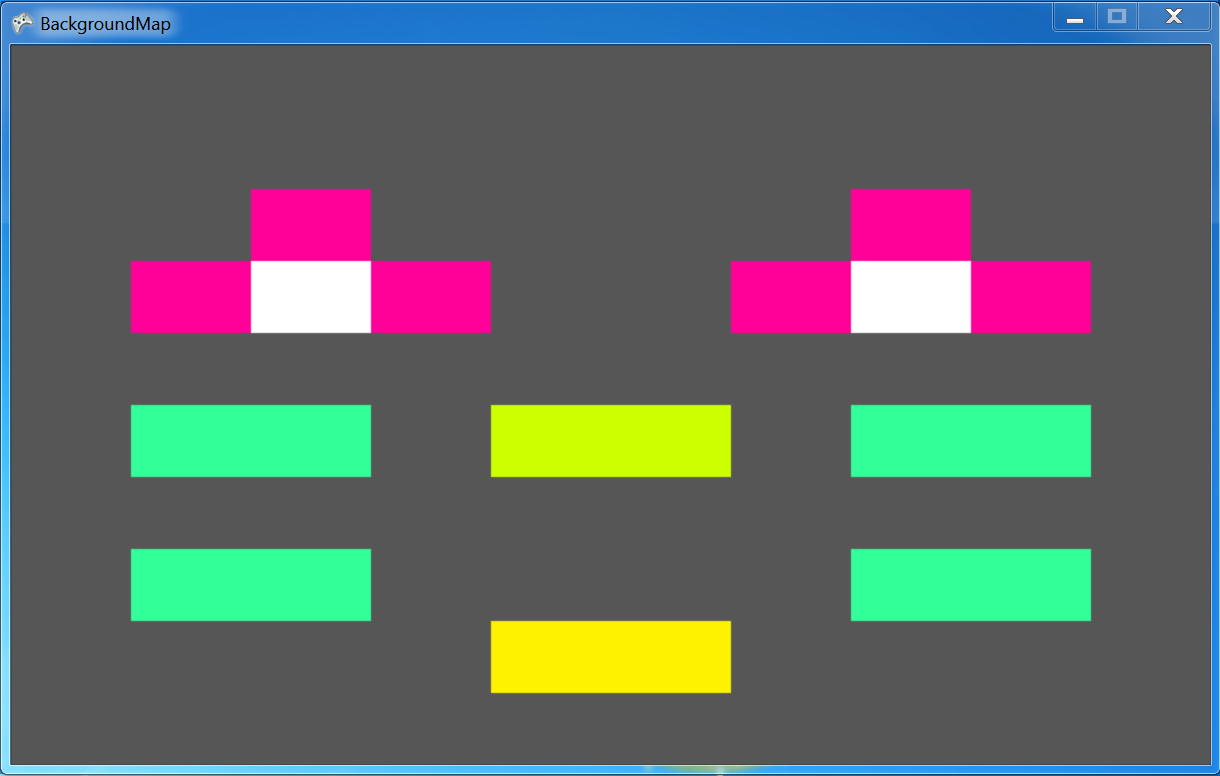
\includegraphics[width=10cm]{../res/mapxna.png}
\end{center}
\caption{Affichage de la carte dans XNA.}
\end{figure}
\end{document}
